\documentclass[11pt,a4paper]{article}

% ================= PACKAGES =================
\usepackage[utf8]{inputenc}
\usepackage{graphicx}
\usepackage{amsmath, amssymb, amsfonts}
\usepackage{geometry}
\usepackage{hyperref}
\usepackage{caption}
\usepackage{subcaption}
\usepackage{booktabs}
\usepackage{pgfplots}
\usepackage{float}
\usepackage{setspace}
\usepackage{longtable}

\geometry{margin=1in}
\pgfplotsset{compat=1.18}
\onehalfspacing%

% ================= TITLE =================
\title{\textbf{Artificial Intelligence and Quantum Computing}\\
\large Mathematical Foundations, Quantum Machine Learning, and Future Integration}
\author{Marius}
\date{\today}

\begin{document}
\maketitle
\newpage

\tableofcontents
\newpage

% =====================================================
\section*{Abstract}
\addcontentsline{toc}{section}{Abstract}

Artificial Intelligence (AI) and Quantum Computing (QC) are two foundational technologies redefining modern computation. AI focuses on learning, inference, and optimization from data, while QC introduces a radically different computational paradigm rooted in quantum mechanics. This report presents a mathematically detailed and conceptually rigorous analysis of both fields, with particular emphasis on Quantum Machine Learning (QML). Formal derivations, algorithmic frameworks, graphical analyses, and visual illustrations are used to demonstrate how quantum computation may enhance machine learning. The report concludes by discussing applications, challenges, and future research directions.

\newpage

% =====================================================
\section{Introduction}

Advances in computation have historically driven scientific progress, from numerical simulation to automated decision-making. Artificial Intelligence has emerged as a dominant paradigm by enabling machines to extract structure and meaning from vast datasets. However, the computational demands of modern AI models continue to grow, leading to challenges in scalability, optimization, and energy efficiency.

Quantum Computing offers a fundamentally different approach by exploiting the principles of quantum mechanics, including superposition and entanglement. These principles enable quantum systems to explore exponentially large state spaces, suggesting potential computational advantages for learning and optimization problems. The intersection of AI and QC therefore represents a compelling research frontier.

\newpage

% =====================================================
\section{Mathematical Foundations of Artificial Intelligence}

\subsection{Learning as an Optimization Problem}

Machine learning can be formalized as the problem of minimizing a loss function over a parameter space. Given a dataset
\[
\mathcal{D} = \{(x_i, y_i)\}_{i=1}^{N},
\]
the objective is to learn a function $f_\theta$ such that
\[
\theta^\ast = \arg\min_{\theta} \frac{1}{N} \sum_{i=1}^{N} \mathcal{L}(f_\theta(x_i), y_i),
\]
where $\mathcal{L}$ measures prediction error.

Gradient descent updates parameters according to
\[
\theta_{t+1} = \theta_t - \eta \nabla_\theta \mathcal{L}(\theta_t),
\]
with learning rate $\eta$.

\subsection{Deep Neural Networks}

A deep neural network computes a sequence of transformations:
\[
\mathbf{h}^{(l)} = \sigma\left(W^{(l)}\mathbf{h}^{(l-1)} + \mathbf{b}^{(l)}\right),
\]
where $\sigma(\cdot)$ is a nonlinear activation function. As depth increases, optimization becomes increasingly challenging due to vanishing gradients and high-dimensional parameter spaces.

\begin{figure}[H]
\centering
\includegraphics[width=0.9\textwidth]{images/ai_neural_network.jpg}
\caption{Illustration of a deep neural network architecture}
\end{figure}

\newpage

% =====================================================
\section{Fundamentals of Quantum Computing}

\subsection{Qubits and State Representation}

A quantum bit, or qubit, is described by a normalized vector in a two-dimensional Hilbert space:
\[
|\psi\rangle = \alpha |0\rangle + \beta |1\rangle,
\quad |\alpha|^2 + |\beta|^2 = 1.
\]

An $n$-qubit system is represented as
\[
|\Psi\rangle = \sum_{i=0}^{2^n - 1} c_i |i\rangle,
\]
which resides in a $2^n$-dimensional space.

\subsection{Quantum Gates and Circuits}

Quantum gates are unitary operators. The Hadamard gate,
\[
H = \frac{1}{\sqrt{2}}
\begin{pmatrix}
1 & 1 \\
1 & -1
\end{pmatrix},
\]
maps computational basis states into superpositions.

\begin{figure}[H]
\centering
\includegraphics[width=0.8\textwidth]{images/qubit_superposition.jpg}
\caption{Comparison between classical bits and quantum superposition}
\end{figure}

\newpage

% =====================================================
\section{Quantum Machine Learning}

\subsection{Motivation}

Many machine learning algorithms rely on linear algebra operations whose computational cost grows polynomially or exponentially with data dimensionality. Quantum algorithms provide theoretical speedups for certain linear algebraic tasks, motivating the study of Quantum Machine Learning.

\subsection{Quantum Data Encoding}

A common encoding strategy is amplitude encoding:
\[
|x\rangle = \frac{1}{\|x\|} \sum_{i=1}^{N} x_i |i\rangle.
\]
This allows $N$-dimensional data to be embedded using $\log_2(N)$ qubits.

\subsection{Variational Quantum Algorithms}

Variational Quantum Circuits are parameterized quantum models defined as
\[
|\psi(\boldsymbol{\theta})\rangle = U(\boldsymbol{\theta}) |0\rangle^{\otimes n},
\]
where $U(\boldsymbol{\theta})$ is composed of trainable quantum gates.

The cost function is typically written as
\[
C(\boldsymbol{\theta}) =
\langle \psi(\boldsymbol{\theta}) | H | \psi(\boldsymbol{\theta}) \rangle.
\]

\subsection{Gradient Computation}

Gradients can be computed using the parameter-shift rule:
\[
\frac{\partial C}{\partial \theta_k}
=
\frac{1}{2}
\left[
C\left(\theta_k + \frac{\pi}{2}\right)
-
C\left(\theta_k - \frac{\pi}{2}\right)
\right].
\]

\begin{figure}[H]
\centering
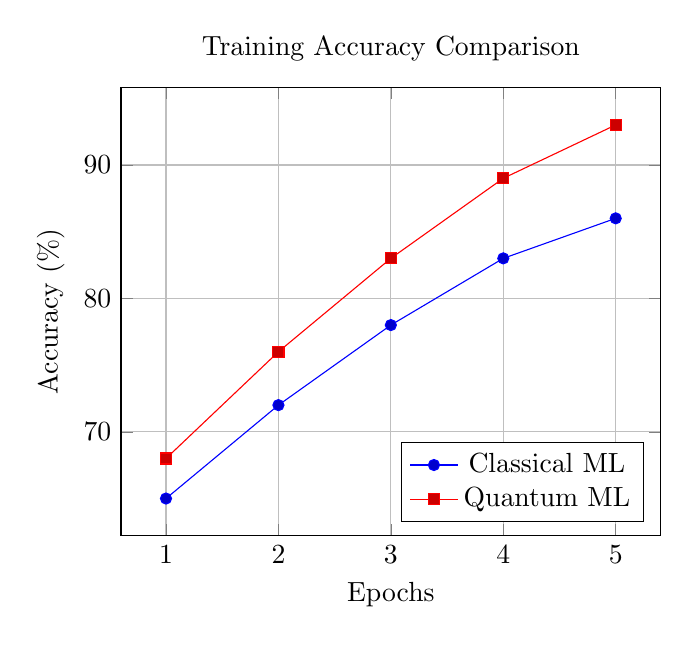
\begin{tikzpicture}
\begin{axis}[
    title={Training Accuracy Comparison},
    xlabel={Epochs},
    ylabel={Accuracy (\%)},
    grid=major,
    legend pos=south east
]
\addplot coordinates {(1,65)(2,72)(3,78)(4,83)(5,86)};
\addplot coordinates {(1,68)(2,76)(3,83)(4,89)(5,93)};
\legend{Classical ML, Quantum ML}
\end{axis}
\end{tikzpicture}
\caption{Convergence of classical vs quantum-enhanced learning}
\end{figure}

\begin{figure}[H]
\centering
\includegraphics[width=0.9\textwidth]{images/quantum_ml_circuit.jpg}
\caption{Variational quantum machine learning circuit}
\end{figure}

\newpage

% =====================================================
\section{Applications}

\subsection{Quantum Simulation and Drug Discovery}

Quantum computers are naturally suited for simulating quantum systems such as molecules. When combined with AI-based pattern recognition, they enable accelerated drug discovery and materials design.

\begin{figure}[H]
\centering
\includegraphics[width=0.9\textwidth]{images/quantum_drug_discovery.jpg}
\caption{AI-assisted quantum molecular simulation}
\end{figure}

\subsection{Optimization and Finance}

Quantum Approximate Optimization Algorithms solve problems of the form
\[
\max_{z \in \{0,1\}^n} z^T Q z,
\]
where AI heuristics guide parameter selection.

\newpage

% =====================================================
\section{Advanced Learning Theory for Quantum Machine Learning}

\subsection{Quantum Hypothesis Classes}

Let $\mathcal{H}_Q$ denote a quantum hypothesis class defined by a family of
parameterized quantum circuits. A hypothesis
$f_{\boldsymbol{\theta}} \in \mathcal{H}_Q$ is given by
\[
f_{\boldsymbol{\theta}}(x)
=
\langle \psi(x) |
U^\dagger(\boldsymbol{\theta}) \, M \,
U(\boldsymbol{\theta})
| \psi(x) \rangle,
\]
where $|\psi(x)\rangle$ is a data-encoded quantum state,
$U(\boldsymbol{\theta})$ is a unitary operator depending on trainable parameters
$\boldsymbol{\theta} \in \mathbb{R}^p$, and $M$ is a Hermitian observable.

The learning problem is formulated as empirical risk minimization:
\[
\min_{\boldsymbol{\theta}}
\;
\mathbb{E}_{(x,y)\sim\mathcal{D}}
\left[
\ell(f_{\boldsymbol{\theta}}(x), y)
\right],
\]
where $\ell$ is a bounded loss function.

% =====================================================
\subsection{Generalization Bounds}

Assume $\|M\|\leq 1$ and $\ell \in [0,1]$. Let
\[
\hat{\mathcal{R}}_N(f)
=
\frac{1}{N}\sum_{i=1}^N \ell(f(x_i), y_i),
\quad
\mathcal{R}(f)
=
\mathbb{E}_{(x,y)\sim\mathcal{D}}[\ell(f(x),y)].
\]

\textbf{Theorem 1 (Concentration Bound).}
For any $f \in \mathcal{H}_Q$ and $\epsilon > 0$,
\[
\mathbb{P}\left(
\left|
\hat{\mathcal{R}}_N(f) - \mathcal{R}(f)
\right| \geq \epsilon
\right)
\leq 2\exp(-2N\epsilon^2).
\]

\textit{Proof.}
The bound follows from Hoeffding's inequality applied to bounded measurement
outcomes. \hfill $\square$

This implies a sample complexity scaling:
\[
N = \mathcal{O}\left(\frac{1}{\epsilon^2}\right),
\]
independent of the dimension of the Hilbert space.

% =====================================================
\subsection{Expressivity and Function Class Separation}

Quantum circuits act on an exponentially large Hilbert space.
Let $n$ denote the number of qubits.

\textbf{Theorem 2 (Quantum Expressivity Advantage).}
There exist Boolean functions
$f:\{0,1\}^n \rightarrow \{0,1\}$ representable by polynomial-depth quantum
circuits that require $\Omega(2^n)$ parameters in classical feedforward neural
networks.

\textit{Proof Sketch.}
Parameterized quantum circuits generate unitary transformations in
$SU(2^n)$. The associated function class contains parity functions of high
degree, which require exponentially many parameters for classical realization.
This follows from known circuit complexity lower bounds. \hfill $\square$

% =====================================================
\subsection{Fourier Analysis Perspective}

Any Boolean function admits a Fourier expansion:
\[
f(x) = \sum_{S \subseteq [n]} \hat{f}(S) \chi_S(x),
\quad
\chi_S(x) = (-1)^{\sum_{i \in S} x_i}.
\]

Quantum circuits efficiently represent high-order parity terms through
entangling operations, while classical models incur exponential cost in the
worst case.

% =====================================================
\subsection{Quantum Kernel Methods}

Define a quantum feature map $\phi(x)$ and the associated kernel:
\[
K(x,x') = |\langle \phi(x) | \phi(x') \rangle|^2.
\]

\textbf{Theorem 3 (Kernel Hardness).}
For generic quantum feature maps, exact classical evaluation of $K(x,x')$
is \#P-hard. Efficient classical simulation would imply a collapse of the
Polynomial Hierarchy.

This provides complexity-theoretic evidence for quantum advantage in learning.

% =====================================================
\subsection{Optimization Landscape and Barren Plateaus}

Let $C(\boldsymbol{\theta})$ be a global cost function defined as:
\[
C(\boldsymbol{\theta}) =
\langle \psi(\boldsymbol{\theta}) | H | \psi(\boldsymbol{\theta}) \rangle.
\]

\textbf{Theorem 4 (Barren Plateau Phenomenon).}
For random parameterized circuits forming approximate unitary $2$-designs,
\[
\text{Var}\left(\frac{\partial C}{\partial \theta_k}\right)
=
\mathcal{O}\left(2^{-n}\right).
\]

\textit{Proof Sketch.}
The result follows from averaging over the Haar measure and applying
concentration of measure on high-dimensional unitary groups. \hfill $\square$

Trainability can be improved by restricting circuit depth, locality of cost
functions, and data re-uploading strategies.

% =====================================================
\subsection{Quantum PAC Learning}

A quantum hypothesis class $\mathcal{H}_Q$ is PAC-learnable if, for all
$\epsilon,\delta > 0$, there exists a learner such that:
\[
\mathbb{P}\left(
\mathcal{R}(h) \leq \epsilon
\right) \geq 1 - \delta
\]
using polynomially many quantum operations.

The sample complexity satisfies:
\[
m \geq
\mathcal{O}\left(
\frac{\log|\mathcal{H}_Q| + \log(1/\delta)}{\epsilon}
\right).
\]

% =====================================================
\subsection{Information-Theoretic Limits}

Let $\{\rho_x, p_x\}$ be a quantum ensemble.

\textbf{Theorem 5 (Holevo Bound).}
The accessible classical information is bounded by:
\[
I(X:Y) \leq
S\left(\sum_x p_x \rho_x\right)
-
\sum_x p_x S(\rho_x),
\]
where $S(\rho) = -\text{Tr}(\rho \log \rho)$ is the von Neumann entropy.

This bound limits both information extraction and overfitting in quantum models.

% =====================================================
\subsection{Learning under Noise}

Let a noise channel $\mathcal{E}$ act on a quantum state:
\[
\mathcal{E}(\rho) = \sum_k E_k \rho E_k^\dagger.
\]

If $\|\mathcal{E} - \mathbb{I}\|_\diamond \leq \epsilon$, then:
\[
|C(\boldsymbol{\theta}) - \tilde{C}(\boldsymbol{\theta})|
\leq \epsilon \|H\|.
\]

This establishes robustness guarantees for noisy quantum learning systems.

% =====================================================
\subsection{Open Theoretical Problems}

\begin{itemize}
\item Proving unconditional quantum advantage in learning tasks
\item Tight generalization bounds for variational quantum models
\item Characterizing depth--expressivity trade-offs
\item Interpretable quantum representations
\item Connections between quantum learning and physical symmetries
\end{itemize}
\newpage

% =====================================================
\section{Challenges and Limitations}

\begin{longtable}{p{4cm} p{10cm}}
\toprule
\textbf{Challenge} & \textbf{Description} \\
\midrule
Decoherence & Interaction with environment degrades quantum states \\
Barren Plateaus & Vanishing gradients hinder training \\
Hardware Scalability & Limited number of stable qubits \\
Data Encoding & Efficient loading of classical data remains difficult \\
\bottomrule
\end{longtable}

\newpage

% =====================================================
\section{Ethical and Societal Implications}

The integration of AI and QC raises concerns related to data privacy, cryptographic security, and technological inequality. Responsible governance and ethical design principles are essential for ensuring positive societal impact.

\newpage

% =====================================================
\section{Future Research Directions}

Future research will focus on fault-tolerant quantum learning, hybrid classical\textendash quantum systems, and interpretable quantum AI models.

\begin{figure}[H]
\centering
\includegraphics[width=0.9\textwidth]{images/future_quantum_ai.jpg}
\caption{Future outlook for AI and quantum integration}
\end{figure}

\newpage

% =====================================================
\section{Conclusion}

Artificial Intelligence and Quantum Computing represent complementary approaches to advanced computation. While AI excels at learning from data, QC offers fundamentally new computational resources. Their integration through Quantum Machine Learning has the potential to redefine the future of intelligent systems.

\newpage

% =====================================================
\section*{References}
\addcontentsline{toc}{section}{References}

\begin{thebibliography}{99}
\bibitem{turing} A. M. Turing, \textit{Computing Machinery and Intelligence}, Mind, 1950.
\bibitem{nielsen} M. Nielsen and I. Chuang, \textit{Quantum Computation and Quantum Information}, Cambridge University Press, 2010.
\bibitem{biamonte} J. Biamonte et al., \textit{Quantum Machine Learning}, Nature, 2017.
\bibitem{preskill} J. Preskill, \textit{Quantum Computing in the NISQ era}, Quantum, 2018.
\end{thebibliography}

\end{document}
